
\noindent

%_ Multidisciplinary Project
\begin{minipage}{\dimexpr 0.5\textwidth-2pt\relax}
    \begin{twmnotebook}[\linewidth]{Multidisciplinary\_Project\_AI\_Oriented.md}[0pt][height=325pt]
\textcolor{chillblue}{Project: Full-Pipeline Acrobatic Drone based on Latent Imitation Learning}\\
\textbullet \quad \textcolor{chillgreen}{Latent Imitation Learning:} Trains an AI model to imitate expert pilot behavior using latent space representations and performance-based evaluation, enabling policies that can potentially surpass the original demonstrations.\\
\textbullet \quad \textcolor{chillgreen}{Goal:} framework designed to act as an "AI Co-pilot," denoising erratic, suboptimal human inputs into safe, expert-level 3D trajectories.\\
\textbullet \quad \textcolor{chillgreen}{Main components:} Gazebo Harmonic for simulation and physics, PX4 Autopilot for high-frequency flight control (400Hz), Micro XRCE-DDS for PX4-ROS2 communication, and ROS2 as the offboard middleware handling sensors, messaging, and AI integration (80Hz). The acrobatic AI runs as a Python ROS2 node at a lower control frequency (0.5Hz). \hypertarget{drone}{}\\
\textbullet \quad \textcolor{chillgreen}{Principle:} Inputs include raw human control commands, telemetry data, and environmental perception data (vision and 3D sensing). The AI generates an intended trajectory through the environment, which is validated by a safety and obstacle-avoidance layer before being executed by PX4 and translated into motor commands.
    \end{twmnotebook}
    \twmhline
    \begin{twmimage}[\dimexpr 0.7\linewidth-2pt\relax]{Test\_Control\_World.png}[height=\dimexpr 125pt - 2pt\relax, valign=center, halign=center]
        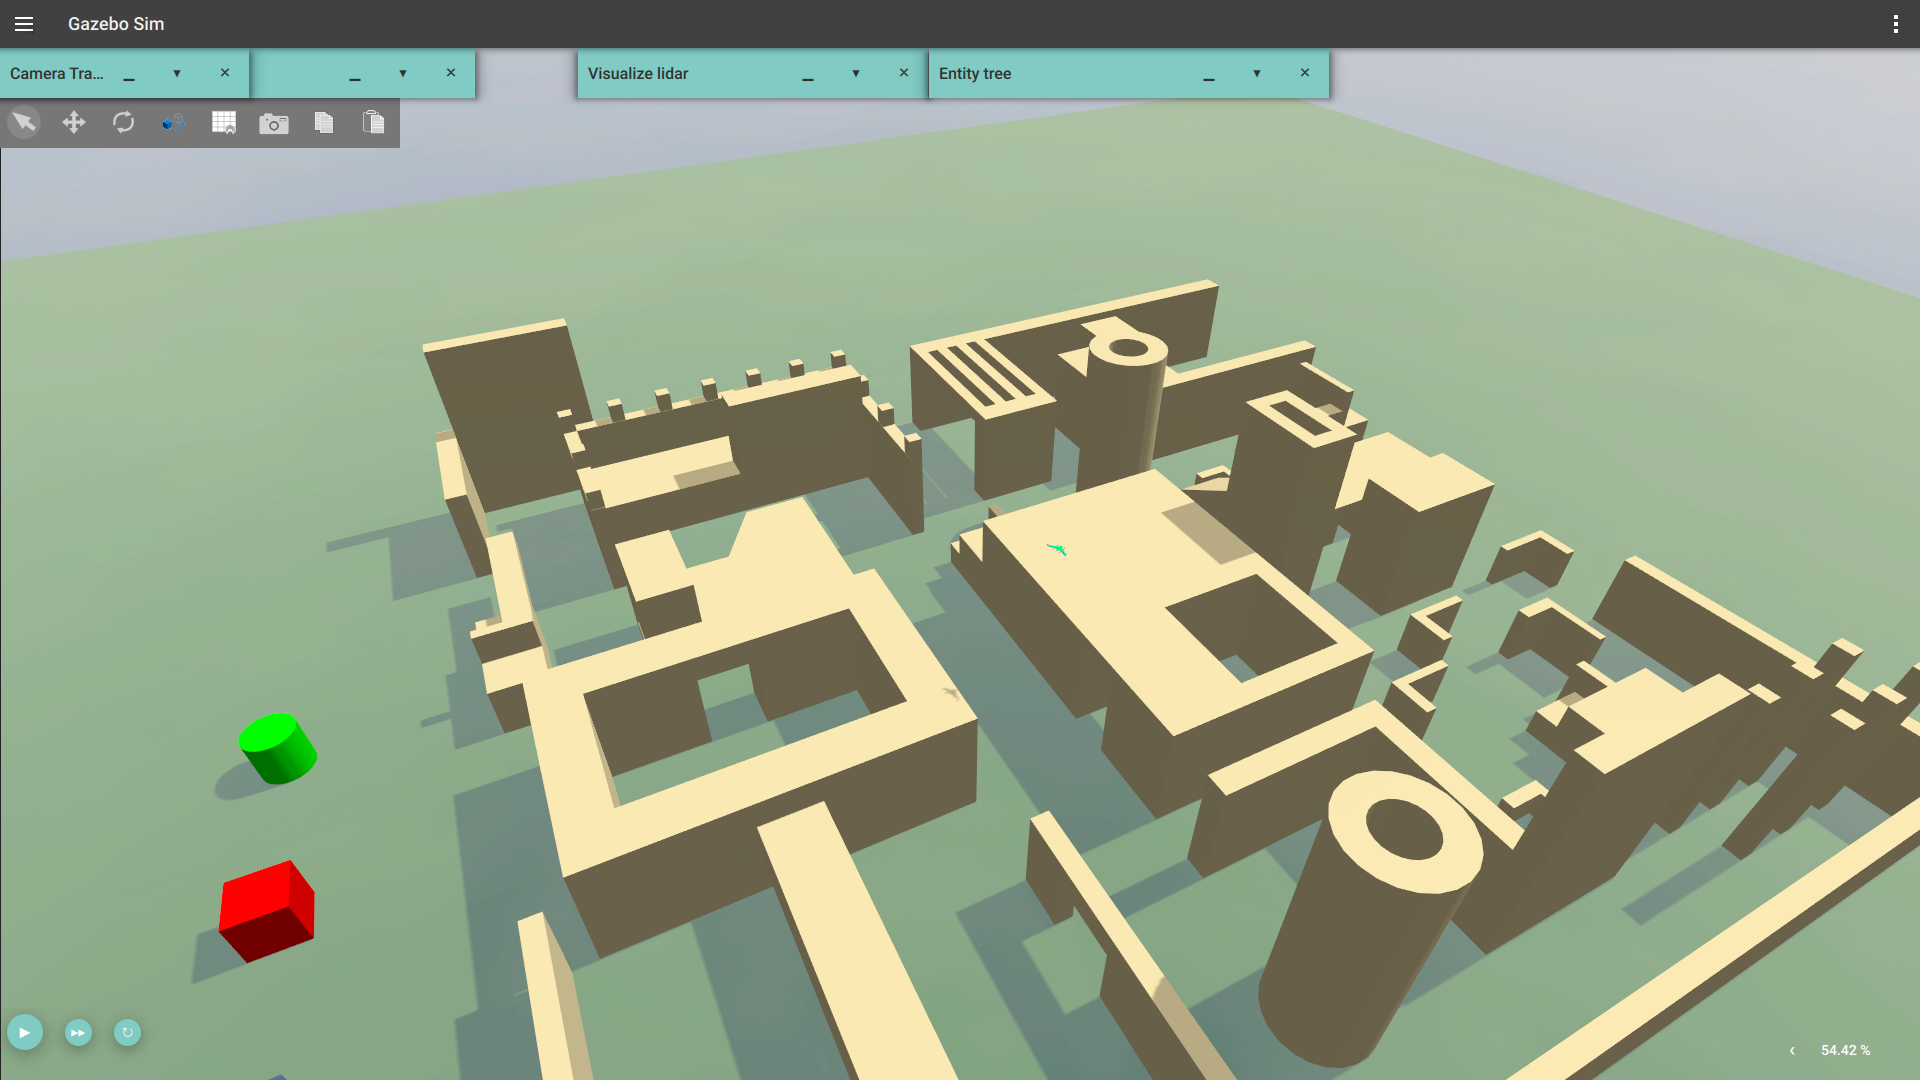
\includegraphics[width=\linewidth, height=\tcbtextheight, keepaspectratio]{figure/test_control_world.png}
    \end{twmimage}%
    \twmgap%_ Replace this with VTOL
    \begin{twmimage}[\dimexpr 0.3\linewidth-2pt\relax]{VTOL.png}[height=\dimexpr 125pt - 2pt\relax, valign=center, halign=center]
        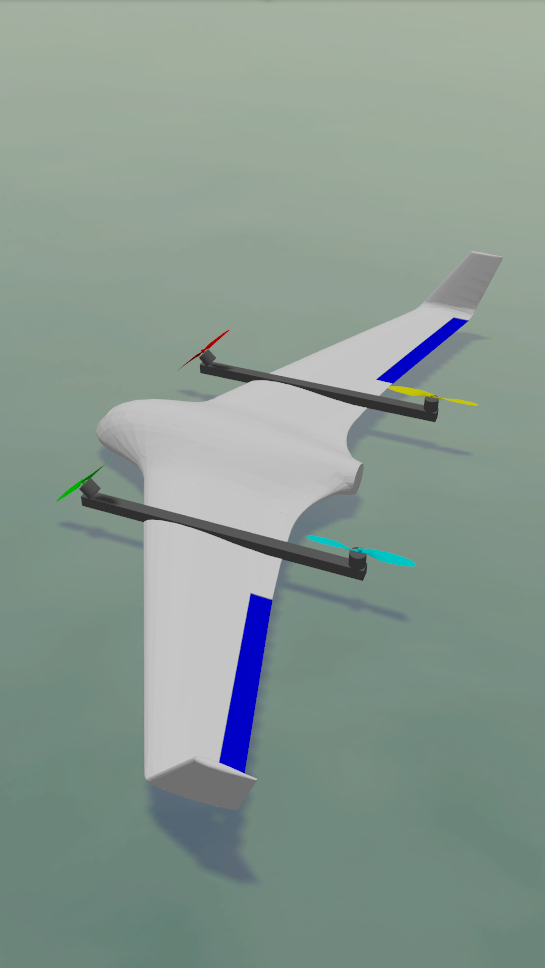
\includegraphics[width=\linewidth, height=\tcbtextheight]{figure/AlphaMinus1_cut.png}
    \end{twmimage}
\end{minipage}%
\twmgap%
\begin{minipage}{\dimexpr 0.5\textwidth-2pt\relax}
    \begin{twmimage}[\dimexpr 0.7\linewidth-2pt\relax]{Test\_non-AI\_behavior.png}[height=\dimexpr 125pt - 2pt\relax, valign=center, halign=center]
        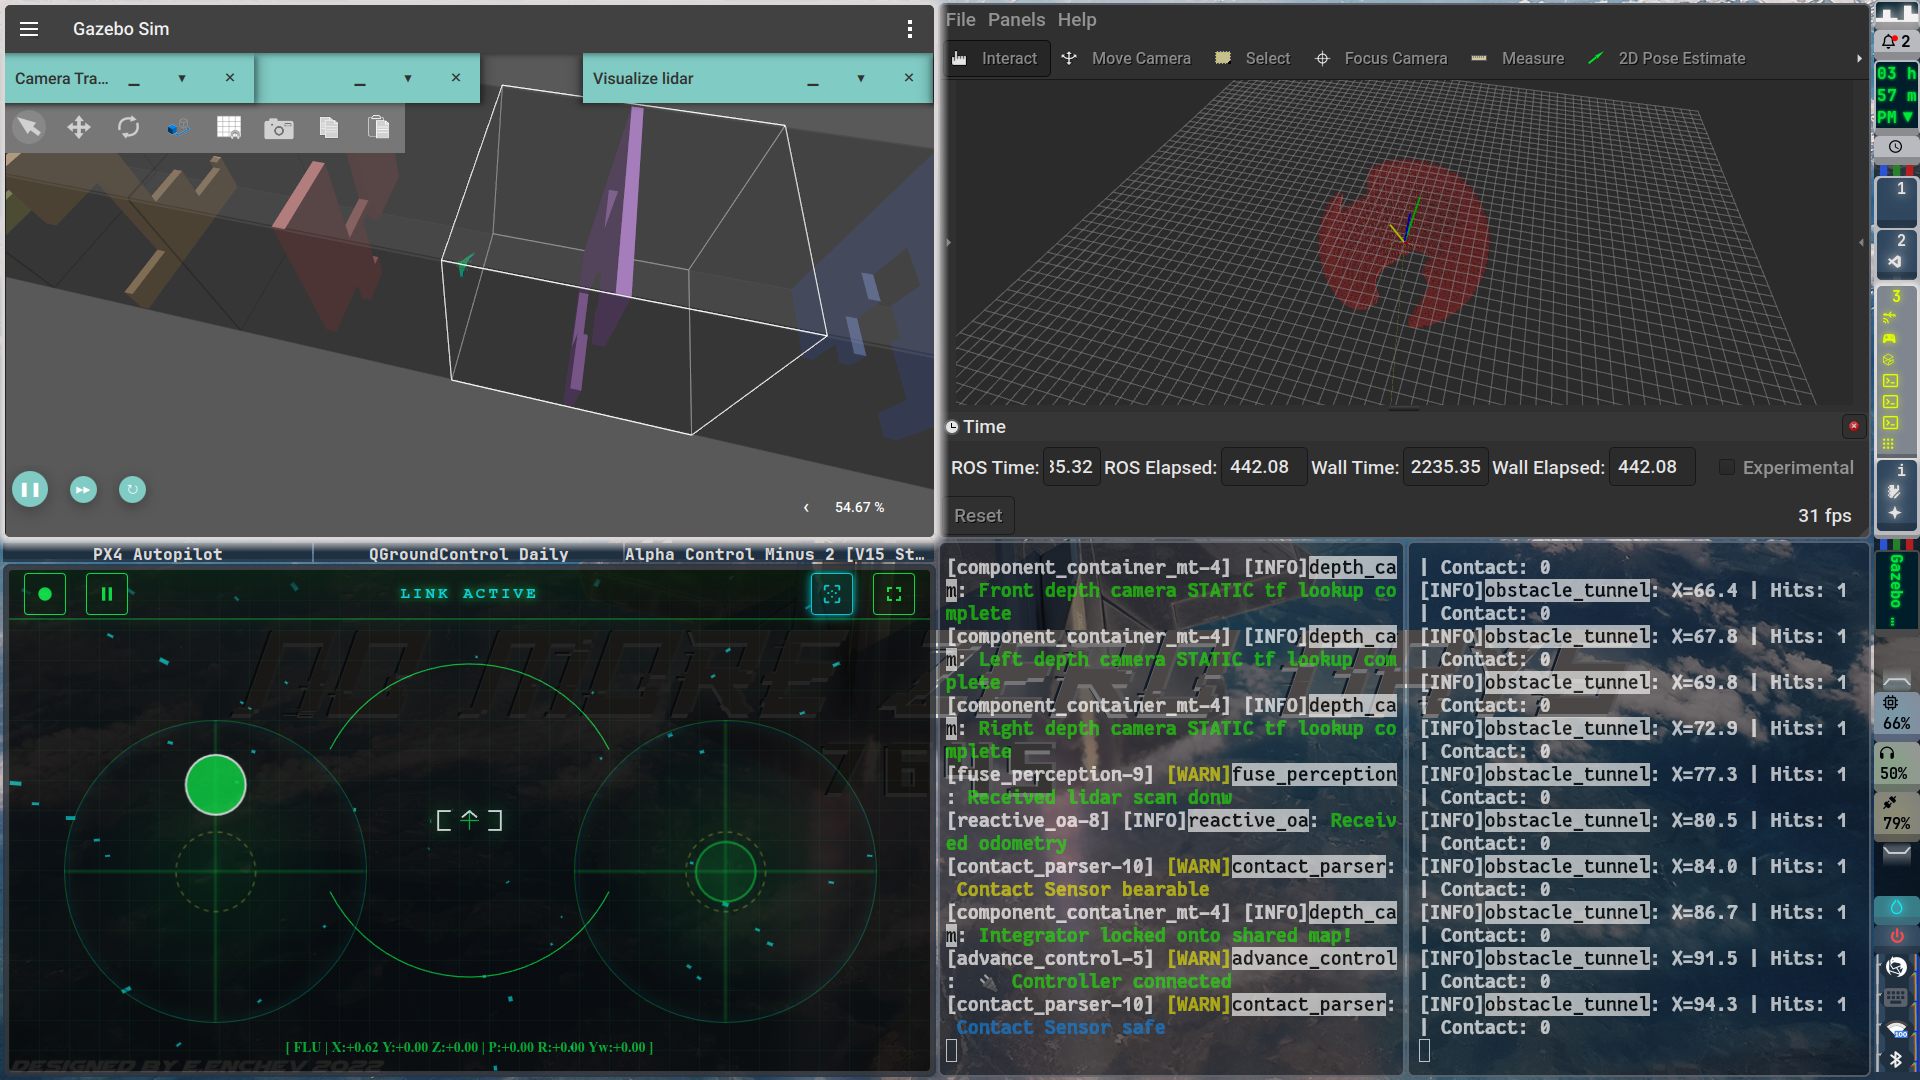
\includegraphics[width=\linewidth, height=\tcbtextheight, keepaspectratio]{figure/DemoDrone2.png}
    \end{twmimage}%
    \twmgap%
    \begin{twmimage}[\dimexpr 0.3\linewidth-2pt\relax]{Pipeline.png}[height=\dimexpr 125pt - 2pt\relax, valign=center, halign=center]
        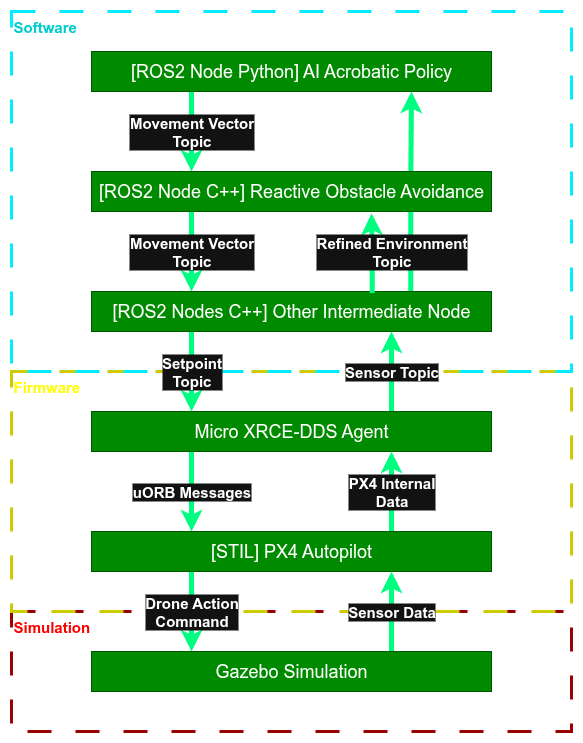
\includegraphics[width=\linewidth, height=\tcbtextheight, keepaspectratio]{figure/OverviewPipeline.png}
    \end{twmimage}
    \twmhline
    \begin{twmnotebook}[\linewidth]{Multidisciplinary\_Project\_AI\_Oriented.md}[0pt][height=325pt]
\textbullet \quad \textcolor{chillgreen}{Execution:} Collected expert control inputs and telemetry data in Gazebo to build a training dataset. The simulation environment consisted of a procedurally generated obstacle-tunnel world. Models were trained offline and evaluated through both offline testing and real-time user-controlled flight scenarios.\\
\textbullet \quad \textcolor{chillgreen}{Results:} Successfully validated the non-AI control pipeline, including low-level obstacle avoidance, achieving autonomous flights of up to 1 km without collisions. However, the AI-controlled system produced noisy outputs and occasionally conflicted with user inputs, resulting in unstable flight behavior. Simulated latency average 290us\\
\textbullet \quad \textcolor{chillgreen}{Diagnosed:} Early model outputs revealed limitations in the design and data flow between high and low layers, indicated the need for an improved model and larger training datasets.\\
\textbullet \quad \textcolor{chillgreen}{Future:} Currently redesigning the pipeline with a focus on low-level data processing, system integration, and control structures to support more dynamic acrobatic maneuvers.\\
\textbullet \quad \textcolor{chillgreen}{Summarize:} Demonstrated the feasibility of the overall control pipeline. Further refinement of both the AI and robotics architectures is needed.
    \end{twmnotebook}
\end{minipage}

\twmhline

%_ Internship Project
\begin{twmnotebook}[\dimexpr 0.5\textwidth-2pt\relax]{Internship\_Work.md}[0pt][height=340pt]
    \textcolor{chillblue}{Project: Cross-Platform ITAM Endpoint Device Agent}\\
    \textbullet \quad \textcolor{chillgreen}{Goal:} Develop a lightweight, memory-safe IT asset monitoring daemon for Linux and Windows.\\
    \textbullet \quad \textcolor{chillgreen}{Main components:} Rust, Tokio, Unix Domain Sockets, Min-Heap scheduler, flamegraph, hyperfine.\\
    \textbullet \quad \textcolor{chillgreen}{Principle:} Architecture is decoupled into discrete binaries (launcher, worker, fetcher) linked by IPC. This isolates faults-a fetcher panic will not crash the main daemon. Precise task scheduling is managed via a custom Min-Heap scheduler.\\
    \textbullet \quad \textcolor{chillgreen}{Execution:} Built the multi-binary Rust agent handling OS-specific system calls. Implemented the IPC layer for data passing and profiled memory/CPU bottlenecks using flamegraphs and hyperfine.\\
    \textbullet \quad \textcolor{chillgreen}{Results:} Successfully delivered a functioning cross-platform agent capable of scheduled data fetching and resilient inter-process communication without memory leaks.\\
    \textbullet \quad \textcolor{chillgreen}{Summarize:} Delivered a foundational MVP, successfully demonstrating Rust's utility as a highly effective choice for building memory-safe, low-overhead system architectures.
\end{twmnotebook}%
\twmgap%_ Capstone Project
\begin{twmnotebook}[\dimexpr 0.5\textwidth-2pt\relax]{Capstone\_Project\_Plan.md}[0pt][height=340pt]
    \textcolor{chillblue}{Project: VTOL Acrobatic Control \& Twin Obstacle Avoidance Architecture}\\
    \textcolor{chillgreen}{Goals:} Design an AI-driven control pipeline that explores and exploits the highly non-linear flight envelope of VTOL while maintaining deterministic spatial safety.\\
    \textcolor{chillgreen}{Main components:} C++, ROS2 (Jazzy), PyTorch (RL), Mixture of Experts (MoE), Voxblox (ESDF), Gazebo Harmonic, PX4 Autopilot.\\
    \textcolor{chillgreen}{Principle:} Engineered a "Twin OA" architecture. The Acrobatic OA utilizes a Reinforcement Learning Mixture of Experts (MoE) network—featuring hardware-specific experts and a mixing layers—to generate complex actuator sequences and predicted states. These probabilistic AI outputs are strictly validated by the Reactive OA, which performs deterministic collision checks using a continuous Voxblox ESDF map. Validated states bypass the rigid PX4 mixer for direct acrobatic execution, while rejected states instantly trigger a spatial safety fallback.\\
    \textcolor{chillgreen}{Summarize:} Proposing a novel, mathematically validated AI architecture designed to safely push VTOL hardware to its aerodynamic limits without relying on static control mixers.
\end{twmnotebook}


